\RequirePackage{luatex85}
\documentclass[tikz]{standalone}
\begin{document}

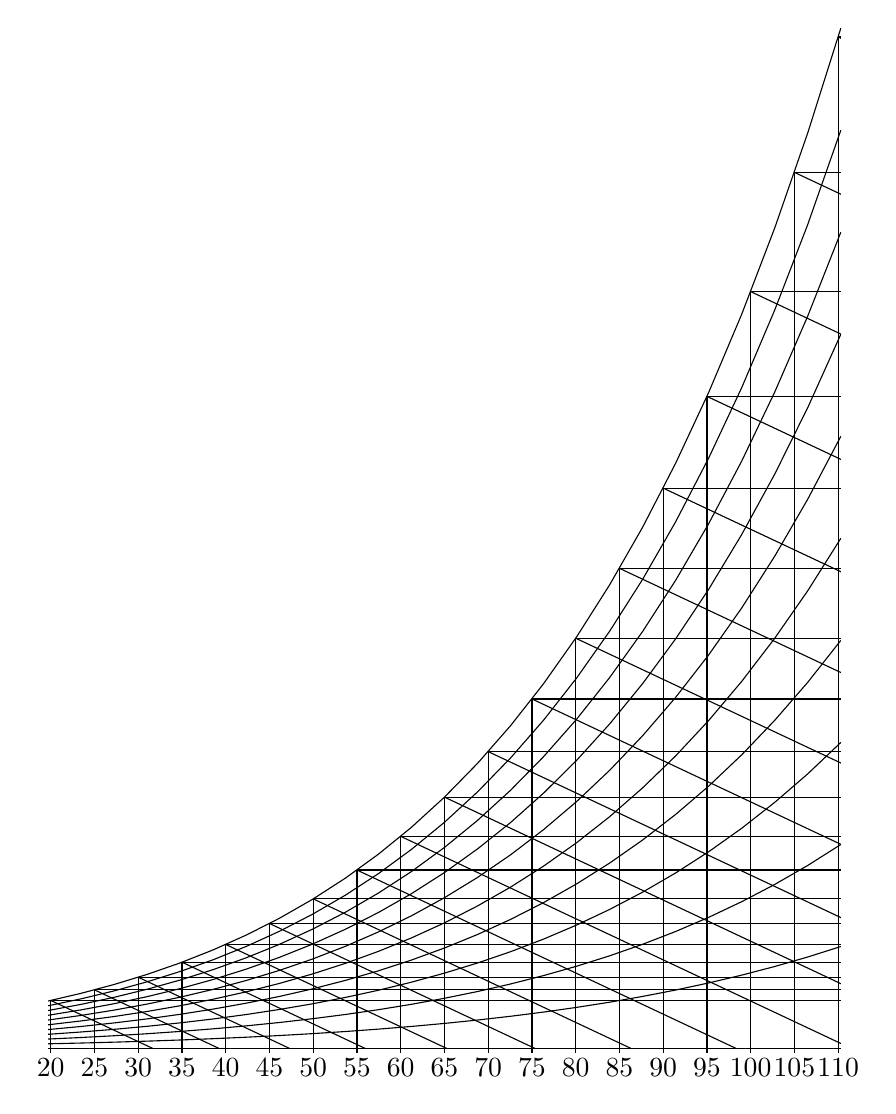
\begin{tikzpicture}[domain=19.7:110.3, scale=0.2]
\foreach \y in {1,...,10} \draw
	plot ({(\x-32)/1.8+273}, 
		{0.1*\y*exp(20.386-5132/((\x-32)/1.8+273))});
\draw ({(19.7-32)/1.8+273},0) 
	-- ({(110.3-32)/1.8+273},0);
\foreach \x in {20,25,...,110} \draw
	({(\x-32)/1.8+273},0) node[below] {\x};
\clip ({(19.7-32)/1.8+273},-0.3) rectangle 
	({(110.3-32)/1.8+273},
		{exp(20.386-5132/((110.3-32)/1.8+273))});
\foreach \x in {20,25,...,110} \draw
	({(\x-32)/1.8+273},
		{exp(20.386-5132/((\x-32)/1.8+273))})
	edge[-] ({(110.3-32)/1.8+273)},
		{exp(20.386-5132/((\x-32)/1.8+273))})
	edge[-] ({(\x-32)/1.8+273
		+2.125*exp(20.386-5132/((\x-32)/1.8+273)))},0)
	edge[-] ({(\x-32)/1.8+273)},-0.3)
	;
\end{tikzpicture}

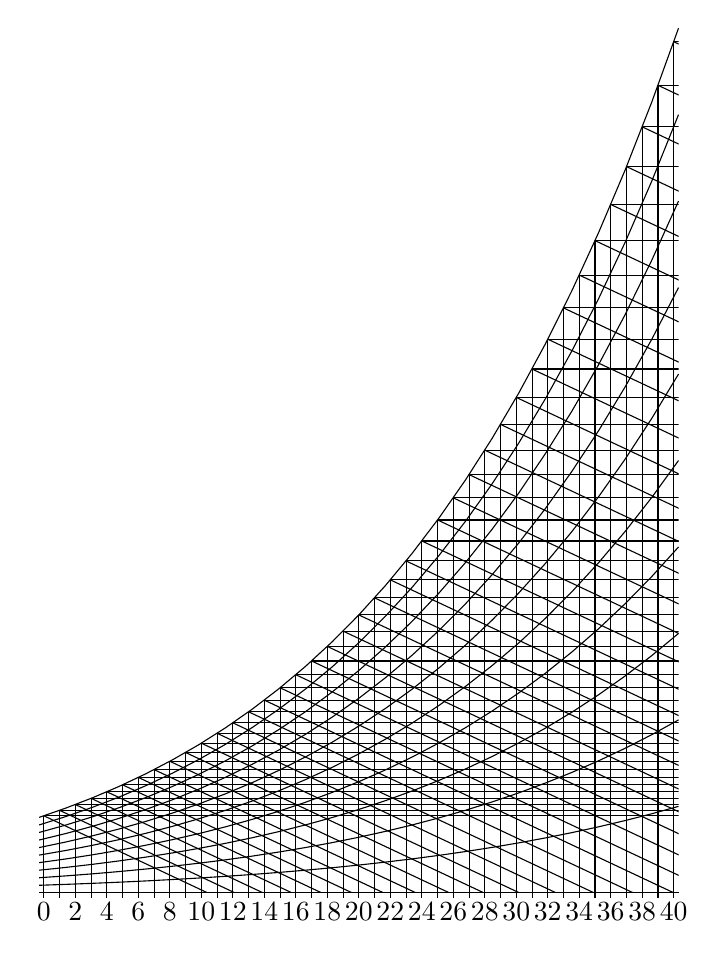
\begin{tikzpicture}[domain=272.7:313.3, scale=0.2]
\foreach \y in {1,...,10} \draw
	plot (\x, {0.1*\y*exp(20.386-5132/\x)});
\draw ({273-0.3},-0.3) grid ({273+40+0.3},+0.3);
\foreach \x in {0,2,...,40} \draw
	(\x+273,0) node[below] {\x};
\clip (272.7,0) rectangle 
	(313.3,{exp(20.386-5132/313.3)});
\foreach \x in {0,...,40} \draw
	(\x+273,{exp(20.386-5132/(\x+273))})
	edge[-] (313+0.3,{exp(20.386-5132/(\x+273))})
	edge[-] ({\x+273+2.125*exp(20.386-5132/(\x+273))},0)
	edge[-] (\x+273,-0.3)
	;
\end{tikzpicture}
\end{document}

2.125=(40-14)/exp(20.386-5132/(273+14))

C*1.8 +32 = F
C = (F-32)/1.8+273